\chapter{Problem Statement} \label{chap:chap3}

In this chapter the problem will be described and justified, using references from the bibliographic study presented in Chapter~\ref{chap:sota}.

The problem statement includes the project's requirements specification, which in turn includes the stakeholder identification. 

A design for the solution is presented, including the UML (Unified Modeling Language) diagram, so that the reasoning behind the solution can be understood. Use cases are also described so that a clear view on what the system does can be obtained. 

The details for the implementation are described in the next chapter (Chapter \ref{chap:chap4} --~\nameref{chap:chap4}).

\section{Problem Description}

Currently, FEUP's computing infrastructures are only accessed by those who have the technical knowledge to interact with the system. These people are technicians whose area of expertise encompasses outsourcing computing resources to perform computing jobs. 

If someone from an area unrelated to the computing system wants to perform any operation in it, that someone must contact the said technicians and waste valuable time trying to find someone that can be of assistance.

Having this in mind, CICA has started developing a project that reduces the amount of knowledge necessary to perform the said computing operations.

This document focuses only on the front-end of the project, the back-end having already been developed by former MIEIC student Nuno Cardoso as part of his Master Thesis. CICA's project is described in greater detail in the following section.

\section{CICA's private cloud project} \label{sec:project}

In this section CICA's private cloud project is described in a greater detail, along with the implemented architectural solution.

The use case scenarios are presented, as well as the UML diagram which shows the entities involved in the web application. As it is customary when designing a software application, a requirements elicitation process was held and the results are also shown in this section.

\subsection{The big picture}\label{subsec:bigpicture}

As it was mentioned earlier in this chapter and in the document, the work depicted in this dissertation is part of a bigger project currently being worked on at CICA (FEUP's Informatics Center).

This project aims at simplifying the process of submitting a computing job into FEUP's computing infrastructures, thus making them more accessible to the academic community, without the users having to spend time learning about the technologies and how the system actually works.

In order to better understand the full extention of the issue, Figure~\ref{fig:big_picture} shows the whole system as it should function, through the means of an hypothetic and yet plausible use case scenario:

\begin{figure}[h!]
  \begin{center}
    \leavevmode
    \fbox{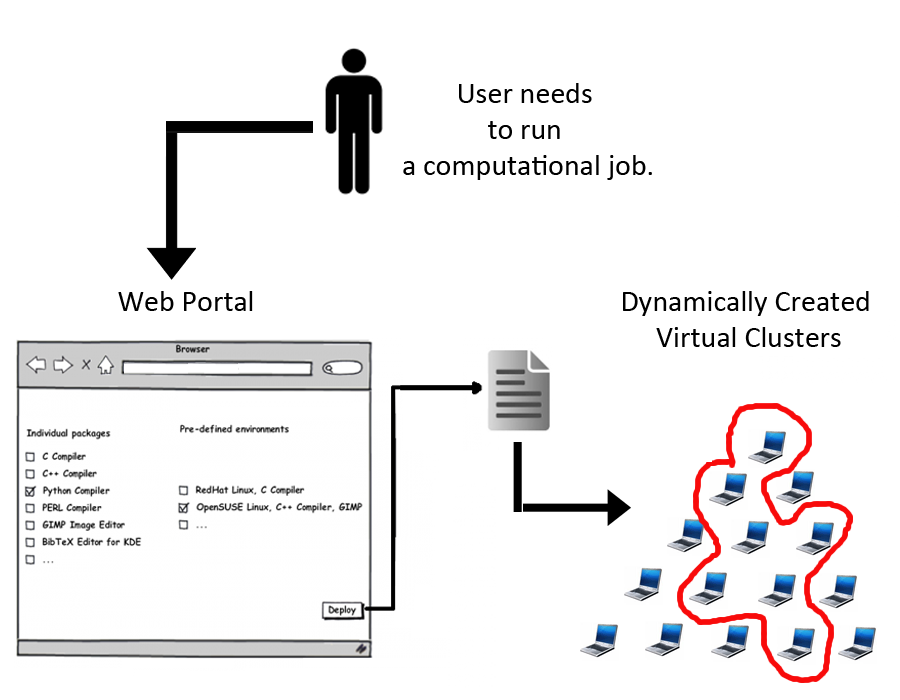
\includegraphics[width=\linewidth]{big_picture.png}}
    \caption{CICA's full computing project.}
    \label{fig:big_picture}
  \end{center}
\end{figure}

Firstly, a researcher of a specific field of study wants to conduct a more complex operation that involves greater computing efforts than his/her home and/or work computer. As such, the researcher proceeds to access the designed system through a web page where he/she can:

\begin{itemize}
	\item Choose a suitable work environment for his/her computational needs according to a set of available options;
	\item Create his/her own work environment according to the specifications he/she provides the system with, namely which programs are needed for the computing job.
\end{itemize}

The system will then automatically create a VM image which will be the environment where the computing job will be run. This VM image will be passed onto the back-end of the project where a virtual cluster will be created according to that virtual environment.

Finally a username and password combination should be returned so that the researcher can enter the created environment and perform his/her operations. 

\subsection{The stakeholders}\label{subsec:stakeholders}

The following stakeholders were identified for this project:

\begin{itemize}
\item FEUP researchers;
\item Web system administrator;
\end{itemize} 

These are the only people or groups of people which will interact with the system.

\subsection{The objectives}\label{subsec:objectives}

Having the project outlined, the following objectives were set:

\begin{enumerate}
\item The web system must be able to create VM images;
\item The VM image creation must be dynamic, i.e. the images must be created according to the users specifications, which are inputted via the web system --- contextualization;
\item The web system must help the users regarding which VM image might be more suitable for their needs by providing the appropriate means for that decision;
\item The web system must provide a way for managing the VM images which were registered in it. This management can be performed by either the users (with limitations) or the system administrator;
\item All the above features must be made transparent for the user (the user does not need to know how things work, as long as they do).
\end{enumerate}

These objectives can be translated into system requirements, which are stated in the next section of this chapter.

\subsection{Requirements specification}\label{subsec:requirements}

As it was mentioned, a software application has certain requirements which must be met so that it complies with the system stakeholders' necessities.

As such, interviews were held with some of these stakeholders in order to understand how the system should behave and what functionalities it should offer.

These requirements can be split in two categories:

\begin{enumerate}
\item Functional requirements --- what the system should do and what functions it should perform~\cite{http://dictionary.reference.com/browse/functional+requirements};
\item Non-functional requirements --- Constraints or restrictions that must be considered when designing the solution~\cite{http://www.requirementsauthority.com/functional-and-non-functional.html}.
\end{enumerate}

\subsubsection{Functional requirements}\label{subsubsec:funct-reqs}

The identified functional requirements are:

\begin{itemize}
\item The system must allow the creation of VM images;
\item This creation must be dynamic -- the user must be able to choose what software is to be installed;
\item The user must be presented with tools which allow him/her to better choose which VM image is better suited for his/her needs or if a new VM image must be created;
\item The VM images must be manageable -- they need to have the option to be modified and/or deleted, as well as located within the web system;
\item The VM image specification within the system must have a certain degree of granularity, so that the previous requirement is able to be met;
\item The system must allow the separation of users -- login system, with different permissions for different users;
\end{itemize}

\subsubsection{Non-functional requirements}\label{subsubsec:nonfunct-reqs}

The identified non-functional requirements are:

\begin{itemize}
\item The system must be intuitive;
\item The system must be as simply designed as possible;
\item Users without specific technical knowledge in computing technologies must be able to use the system.
\end{itemize}

\section{The solution}\label{sec:solution}

In this section the solution is documented and the thought process behind it is justified. An UML diagram is included for better understanding on how the system works. 

\subsection{UML diagram}\label{subsec:uml-diag}

Once the requirements and the stakeholders were defined, a diagram depicting the relations between the different elements in the system was produced and it is shown in figure~\ref{fig:uml-diag}.

\begin{figure}[h]
  \begin{center} 
    \leavevmode 
    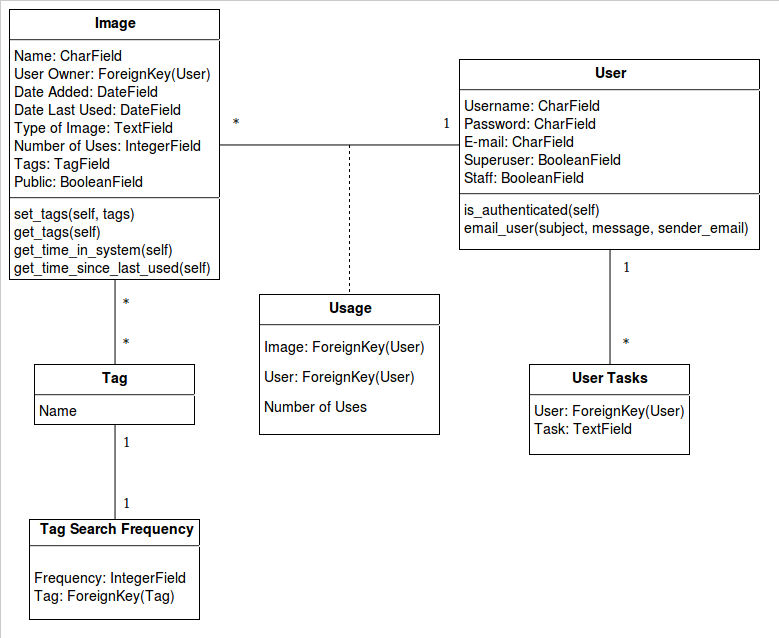
\includegraphics[width=\textwidth]{class_diagram}
    \caption{Entities and their relationship in the system.} 
    \label{fig:uml-diag} 
  \end{center}
\end{figure}

As it can be observed, the following entities are portrayed:

\begin{itemize}
\item Image -- represents the VM images that are created and registered in the system;
\item User -- represents the users that are registered in the system;
\item User Tasks -- represents which task the user has running in the system. This refers to the VM image creation process;
\end{itemize}

The following relationships between the aforementioned entities can be observed:

\begin{itemize}
\item A user can create several VM images, but one image can only have one owner (this, however, does not mean that an image cannot be used by several users);
\item An image can have several ``tags'' and one ``tag'' can by used by several images;
\item A user can have one task running in the system, specifically one creation of a VM image (this is explained in greater detail in the next chapter, \nameref{chap:chap4});
\item A user can use a VM image, this being logged in the system for statistical purposes;
\item The ``tag'' search is also logged for statistical purposes and to help users select a suitable VM image for their needs.
\end{itemize}

\subsection{Use Cases}\label{sec:use-cases}

Alongside the delineation of the entities, relationships and requirements, there is also the need to delineate the use cases for the web system. These describe what actions can be taken inside the web system, either by normal users or the system administrator.

Use case diagrams are used as visual aids for their textual representation and some screenshots are provided. 

\subsubsection{UC1 -- Login into the web system}\label{uc1}

\textbf{Actors}:

\begin{itemize}
\item Researcher/Administrator.
\end{itemize}

\ \\
\textbf{Brief description}:
\ \\
The researcher/administrator (known as ``user'' for the rest of this use case for simplicity) wishes to log into the web system.\\
\ \\
\textbf{Basic flow}:

\begin{itemize}
\item The web system prompts the user for his/her username and password combination (provided beforehand by the system administrator in order to maintain control over who accesses the web system);
\item The user inputs his/her username and password in the boxes provided;
\item The web system validates the entered username and password and logs the researcher/administrator into the system.
\end{itemize}

\ \\
\textbf{Alternative flows}:\\
\ \\
If an incorrect username and password combination is supplied, the page will simply reload. The user must enter a valid username and password combination to proceed.\\
\ \\
\textbf{Pre-conditions}:\\
\ \\
None.\\
\ \\
\textbf{Post-Conditions}:\\
\ \\
If the use case is successful, the user is logged into the system. If the user is a researcher, no special privileges will be gained. If the user is an administrator, ``administrator'' status will be granted and he/she will gain administration privileges over the system.

If the use case is unsuccessful, no changes are made to the system state.

\subsubsection{UC2 -- Perform management operations}\label{uc2}

\textbf{Actors}:

\begin{itemize}
\item System administrator.
\end{itemize}

\ \\
\textbf{Brief description}:\\
\ \\
The system administrator wants to perform management operations in the system.\\
\ \\
\textbf{Basic flow}:

\begin{itemize}
\item In order to perform management operations, the system administrator must login into the system administration panel, which has a different URL from the web system the researchers use;
\item The system administrator must perform the login action as described in the first use case (\nameref{uc1}) using his/her credentials, which are the same for both parts of the system;
\item Inside the administration section, the administrator is able to perform several tasks:
\begin{itemize}
\item Manage the users who can access the web system. This includes adding and deleting users; editing users' details and promoting users to administrators.
\item Manage the database of the system. The administrator can: add VM images to the database; edit VM images' details; and edit or add everything that can be registered by researchers (this may be helpful for testing purposes).
\end{itemize}
\item After the changes are saved, the state of the system is updated.
\end{itemize}

\ \\
\textbf{Alternative flows}:\\
\ \\
None.\\
\ \\
\textbf{Pre-conditions}:\\
\ \\
User must be logged in as administrator.\\
\ \\
\textbf{Post-Conditions}:\\
\ \\
The system state will change to whichever operations the system administrator chose to perform.

\subsubsection{UC3 -- Create a new VM image}\label{uc3}

\textbf{Actors}:

\begin{itemize}
\item Researcher.
\end{itemize}

\ \\
\textbf{Brief description}:\\
\ \\
A researcher wishes to create a new VM image.\\
\ \\
\textbf{Basic flow}:

\begin{itemize}
\item In order to create a new VM image, the researcher must be logged into the system;
\item After a successful login, the researcher must select the appropriate option from the list provided by the web system (``Create a new VM image'');
\item After being redirected to the VM creation page, the researcher must fill in the details for the newly created VM image:
	\begin{itemize}
	\item Name of the VM image;
	\item Tags to be used for the VM image. These should describe the VM image with as much detail as possible so that other users can find it if they need a similar environment;
	\item Mark the image as ``Public'' or not. This will affect whether the VM image will be available for use by other researchers;
	\item Select which packages they wish to install in the new VM.
	\end{itemize}
\item After filling the required details, the researcher must click on the ``Create'' button;
\item The researcher will then be redirected to the ``Post VM image creation'' page which will be refreshed every few minutes so that the VM creation process status can be updated and displayed to the researcher. After the VM is created, the researcher will be prompted on whether the system should launch the VM;
\end{itemize}

\ \\
\textbf{Alternative flows}:\\
\ \\
The VM image name is already in use. In this case the VM image creation will fail and the page will be refreshed so that the VM image details can be filled out one more time.\\
\ \\
\textbf{Pre-conditions}:\\
\ \\
User must be logged in.\\
\ \\
\textbf{Post-Conditions}:\\
\ \\
If the use case is successful, a new VM image will be inserted into the system. If the use case fails, no changes will occur.\\
If the researcher chooses to launch the VM image, he/she will go into the use case~\ref{uc4} ---~\nameref{uc4}.\\

\subsubsection{UC4 -- Launch a VM}\label{uc4}

\textbf{Actors}:

\begin{itemize}
\item Researcher.
\end{itemize}

\ \\
\textbf{Brief description}:\\
\ \\
A researcher wishes to launch a VM.\\
\ \\
\textbf{Basic flow}:

\begin{itemize}
\item In order to launch a VM, the user must be logged in;
\item After a successful login, the researcher has three ways of launching a VM image, depending on whether he/she was the creator of the VM image:
	\begin{itemize}
	\item If he/she created the VM image that he/she wishes to launch, the VM image can be found in either by:
		\begin{itemize} 
		\item The ``User details'' page, which can be accessed anywhere in the system by simply clicking on the name that appears on the top-right corner in every page. In the ``User details'' page the researcher must click the name of the VM image and afterwards click the ``Launch VM'' button;
		\item Clicking the link ``Launch an already existing VM image'' located in the system's index page, which will show the user's created VM images, as well as the VM images in the system which are marked as ``Public''. The researcher will then have to click the VM image's name and click the ``Launch VM'' button displayed in the VM image details's page.
		\end{itemize}
	\item If he/she did not create the VM image, the researcher must search if the VM image is already created (clicking the link ``Search for a VM image'' in the index page of the web system and entering use case~\ref{uc6} --~\nameref{uc6}. If the image is found, the researcher must click on the appropriate link shown in the search results page (the VM image name) which will redirect the researcher to the VM image details' page where a link to launch that VM will be displayed (``Launch VM''), should the VM image be public. If the image is not public, the researcher will have to contact either the VM image creator via the email provided in the search results page or the system administrator.
	\end{itemize}
\item If the researcher clicks the ``Launch VM'' button in the VM image detail's page, he/she will be redirected to the VM launch page, which will display the information regarding the state of the launch. This page will refresh every few seconds and as soon as the VM image is deployed, a warning will be displayed, informing the researcher. The system will also provide the researcher with a username and password combination so that the researcher can access the newly deployed VM.
\end{itemize}

\ \\
\textbf{Alternative flows}:\\
\ \\
The researcher chose to launch a VM after creating it (coming from the use case~\ref{uc3} ---~\nameref{uc3}). In that case the researcher only needs to click the ``Launch VM'' button displayed.\\
\ \\
\textbf{Pre-conditions}:\\
\ \\
User must be logged in.\\
\ \\
\textbf{Post-Conditions}:\\
\ \\
If the use case is successful, a VM image will be deployed and will be ready for use.


\subsubsection{UC5 -- View system wide statistics}\label{uc5}

\textbf{Actors}:

\begin{itemize}
\item Researcher/Administrator.
\end{itemize}

\ \\
\textbf{Brief description}:\\
\ \\
A researcher or administrator (known as ``user'' in this use case for simplicity) wishes to see the system statistics.\\
\ \\
\textbf{Basic flow}:

\begin{itemize}
\item In order to view the system statistics, the user must be logged in;
\item After a successful login, the user can access the system wide statistics by clicking in the appropriate link ``View statistics'';
\item After being redirected to the statistics page, the user is displayed the following information about the system:
	\begin{itemize}
	\item Most used VM images in the system - shows the user the five most used VM images in the system with a clickable VM image name which redirects to the VM image details;
	\item ``Tag'' cloud - visual representation of the ``tag'' usage in the system i.e. the bigger the font used in the ``tag'' name, the higher the usage. In front of the ``tag'' the VM images which contain that ``tag'' are displayed;
	\item ``Tag'' search frequency - shows the user which ``tags'' were searched more frequently.
	\end{itemize}
\item After viewing the statistics, the user can return to the ``Index'' page by clicking the appropriate link.
\end{itemize}

\ \\
\textbf{Alternative flows}:\\
\ \\
None.\\
\ \\
\textbf{Pre-conditions}:\\
\ \\
User must be logged in.\\
\ \\
\textbf{Post-Conditions}:\\
\ \\
None.

\subsubsection{UC6 -- Search for a VM image}\label{uc6}

\textbf{Actors}:

\begin{itemize}
\item Researcher/Administrator.
\end{itemize}

\ \\
\textbf{Brief description}:\\
\ \\
A researcher or administrator (known as ``user'' in this use case for simplicity) wishes to search for a VM image.\\
\ \\
\textbf{Basic flow}:

\begin{itemize}
\item In order to search for an existing VM image, the user must be logged in;
\item After a successful login, the user can search for an existing VM by clicking the appropriate link -- ``Search for a VM image'';
\item After being redirected to the search page, the user must input the search terms he/she wishes to search for. The search terms should be separated by commas (``,'');
\item If the system finds any VM images which are tagged with any of the search terms inputted, these VM images will be displayed in a list with clickable names, which redirect to the VM image details' page.
\end{itemize}

\ \\
\textbf{Alternative flows}:\\
\ \\
Search terms are not found. An error message is displayed and the user is redirected to the search page.\\
\ \\
\textbf{Pre-conditions}:\\
\ \\
User must be logged in.\\
\ \\
\textbf{Post-Conditions}:\\
\ \\
None.


\subsubsection{UC7 -- View the details of an existing VM image}\label{uc7}

\textbf{Actors}:

\begin{itemize}
\item Researcher/Administrator.
\end{itemize}

\ \\
\textbf{Brief description}:\\
\ \\
A researcher or administrator (known as ``user'' in this use case for simplicity) wishes view the details of an existing VM image.\\
\ \\
\textbf{Basic flow}:

\begin{itemize}
\item In order to view the details of an existing VM image, the user must be logged in;
\item After a successful login,  if the user has created that VM image, he/she must click on his/her username displayed in the top-right corner of the page he/she is currently in and select the desired image in the ``Created images'' section of the page;
\item If the user did not create that VM image, he/she has several options for viewing a VM image detail page:
	\begin{enumerate}
	\item Searching for the VM image using the ``Search'' page and going into the use case~\ref{uc6} --~\nameref{uc6};
	\item Going into use case~\ref{uc5} --~\nameref{uc5} -- and click the VM image names displayed in that page;
	\item Clicking the link ``Launch an existing VM image'' in the ``Index'' page and click the names of the VM images displayed in that page.
	\end{enumerate}
\end{itemize}

\ \\
\textbf{Alternative flows}:\\
\ \\
None.\\
\ \\
\textbf{Pre-conditions}:\\
\ \\
User must be logged in.\\
\ \\
\textbf{Post-Conditions}:\\
\ \\
None.

\subsubsection{UC8 -- Modify the details of an existing VM image}\label{uc8}

\textbf{Actors}:

\begin{itemize}
\item Researcher.
\end{itemize}

\ \\
\textbf{Brief description}:\\
\ \\
A researcher wishes to modify the details of an existing VM image.\\
\ \\
\textbf{Basic flow}:

\begin{itemize}
\item In order to modify the details of an existing VM image, the researcher must be logged in and must be the one who created the VM image in question;
\item After a successful login, the researcher must go into use case~\ref{uc7} --~\nameref{uc8}-- and click on his/her username displayed in the top-right corner of the page he/she is currently in and select the desired image in the ``Created images'' section of the page;
\item The researcher must then click the ``Modify VM image'' button and will be redirected to the VM image modification page where he/she will be presented with a form with the details he/she is able to modify;
\item After the user is done updating the desired fields, he/she must click the ``Update'' button.
\end{itemize}

\ \\
\textbf{Alternative flows}:\\
\ \\
The selected VM image is currently being used by another user. The user will not be able to modify the VM image and the use case will fail.\\
\ \\
\textbf{Pre-conditions}:\\
\ \\
User must be logged in and he/she must be the creator of the VM image.\\
\ \\
\textbf{Post-Conditions}:\\
\ \\
VM image details are updated.


\subsubsection{UC9 -- View user details}\label{uc9}

\textbf{Actors}:

\begin{itemize}
\item Researcher.
\end{itemize}

\ \\
\textbf{Brief description}:\\
\ \\
A researcher wishes to view his/her own details.\\
\ \\
\textbf{Basic flow}:

\begin{itemize}
\item In order to view his/her own details, the researcher must be logged in;
\item After a successful login, the researcher must click on his/her name displayed in the top-right corner of any page he/she is in;
\item The researcher will then be redirected to the user details' page.
\end{itemize}

\ \\
\textbf{Alternative flows}:\\
\ \\
None.\\
\ \\
\textbf{Pre-conditions}:\\
\ \\
User must be logged in.\\
\ \\
\textbf{Post-Conditions}:\\
\ \\
None.

\subsubsection{UC10 -- Modify the user's details}\label{uc10}

\textbf{Actors}:

\begin{itemize}
\item Researcher.
\end{itemize}

\ \\
\textbf{Brief description}:\\
\ \\
A researcher wishes to modify his/her own details.\\
\ \\
\textbf{Basic flow}:

\begin{itemize}
\item In order to modify his/her own details, the researcher must be logged in;
\item After a successful login, the researcher must click on his/her name displayed in the top-right corner of any page he/she is in;
\item The researcher will then be redirected to the user details' page;
\item The researcher must then click on the ``Modify'' button;
\item The researcher will be presented with the ``Modify user details'' page which contains a form with the details which are possible to be modified;
\item After the researcher performs the wanted modifications, he/she must click the ``Update'' button.
\end{itemize}

\ \\
\textbf{Alternative flows}:\\
\ \\
None.\\
\ \\
\textbf{Pre-conditions}:\\
\ \\
User must be logged in.\\
\ \\
\textbf{Post-Conditions}:\\
\ \\
User details are updated.

\subsection{Relevant system details}%how this helps the users in choosing a suitable VM?

In this part of the document, relevant system details are presented, namely how the system helps a user in choosing a suitable VM image.\ \\
The Vm image management issue is also addressed, and specifications on how it can be done by an administrator inside the web system is shown.

\subsubsection{Helping the user}


In order to help a user choose a suitable VM image to use for his/her computational job, the following was implemented:

\begin{itemize}
\item A set of statistics was created so the user can see which VM images or ``tags'' are more used across the system (detailed below);
\item A search function so the user can find a VM image by searching for ``tags'' associated with VM images;
\end{itemize}

\ \\
The search function was implemented so that the user can access the system and search for the programs he/she needs to have installed in VM image. If any of the inputted terms match any of the ``tags'' used in a VM image, that VM image will be displayed to the user. Since the system supports multiple ``tag'' search, the user can search for all the terms he/she wishes to and if a VM image containing all the terms searched exists in the system, it will be shown and the user will know that is the suitable environment for his/her needs.\\
\ \\
As for the set of statistics, different types were created:

\begin{enumerate}
\item What VM images the user that is logged in has available to him (this includes public images and those the user created);
\item Which VM images are more used across the system;
\item A ``Tag'' Cloud was created, showing which ``tags'' were most used across the system;
\item Which ``tags'' were most searched across the system.
\end{enumerate}

\ \\
For users who already created a VM image, it is important to know which ones they already created, since they might need to re-use them again.

The most used VM images can be used to identify better created VM images, which can complement the VM image the user had in mind.

Knowing which ``tags'' were more used can help the users identify an environment that was not created yet, an environment that aggregates some of the most used ``tags'' may be helpful for some researchers.

Knowing which ``tags'' were more searched across the system can help the system administrator in knowing if it might be profitable in pinning some of the images ``tagged'' with some of the most searched ``tags'' in the ``Index'' page so that users do not have to spend time searching for something they use regularly.



----> tag cloud <---- falta falar

\subsection{VM image management}\label{subsec:vm-manag}

One of the objectives for this project was that the created VM images can be manageable.

This management can be performed by either a normal user (limited management) or a system administrator.

\subsubsection{Normal users}

A normal user can mark an image for deletion (in case he/she misstyped the image details or realized that the image would not be needed after all).

Another important feature from the system is the possibility of reserving a VM image for later use. If a user knows he/she will need to use a certain VM image in a certain time in the future, he/she can reserve it, by specifying the date when the image will be needed and the system will prevent that image from being deleted.

\subsubsection{System administrators}

System administrators have access to a reserved space inside the system, somewhere that the normal users cannot access (they cannot see it).

In this section of the system, administrators are presented with details that help them manage the VM images registered in the system.

Administrators can see every VM image in the system, as well as for how long they have been registered and how long it has passed since they were last used. 
If a certain time has passed since the image was last used, combining that information with how long they were registered in the system, the administrators are warned of that occurrence and are given the option to eliminate them from the system.

Administrators also can see if a user has marked an image for deletion (in case the user missclicked or misstyped the VM image details) and can choose to eliminate the images from the system.




%Este capítulo deve começar por fazer uma apresentação detalhada do
%problema a resolver\footnote{Na introdução a apresentação do
%  problema foi breve.} podendo mesmo, caso se justifique,
%constituir-se um capítulo com essa finalidade.

%Deve depois dedicar-se à apresentação da solução sem detalhes de
%implementação. 
%Dependendo do trabalho, pode ser uma descrição mais teórica, mais
%``arquitectural'', etc.
%\clearpage
\section{Conclusions}

In this chapter was presented the architecture to be followed in Chapter~\ref{chap:chap4} in the implementation phase. CICA's private cloud project was presented, this document covering the front-end of that project. The objectives were outlined, as well as the use cases and stakeholders.

A model for a solution was also shown, which includes the UML diagram for the current work. This diagram, along with the use cases and stakeholder identification, describe the system to be implemented.

The VM creation and management was successfully implemented.

The project's use cases and stakeholders were also specified.
